\documentclass[runningheads,a4paper]{llncs}

\usepackage[latin1]{inputenc}
\usepackage{graphicx,color,url}
\usepackage[dvips]{epsfig}
\usepackage{verbatim}
\usepackage{tikz}
\usetikzlibrary{shapes,arrows}
\usetikzlibrary{calc,patterns,snakes,decorations.pathmorphing,decorations.markings}
\usetikzlibrary{positioning}

\newcommand{\keywords}[1]{\par\addvspace\baselineskip
\noindent\keywordname\enspace\ignorespaces#1}

\providecommand{\tabularnewline}{\\}

\begin{document}

\mainmatter  % start of an individual contribution

% first the title is needed
\title{Fuzzy Controller for TORCS}
% Antonio - T�tulo provisional, actualizar con el definitivo


% a short form should be given in case it is too long for the running head
\titlerunning{There can be only one}

% the name(s) of the author(s) follow(s) next
%
% NB: Chinese authors should write their first names(s) in front of
% their surnames. This ensures that the names appear correctly in
% the running heads and the author index.
%

%\author{M. Salem \and A.M Mora \and \and J. J. Merelo \inst{1}}
\author{A. N. Onymous\inst{1}%
\thanks{No Institute}}
% Antonio - Los autores que participen
%
\authorrunning{Anonymous, A}
% (feature abused for this document to repeat the title also on left hand pages)

% the affiliations are given next; don't give your e-mail address
% unless you accept that it will be published
%\institute{Dept. of Computer Architecture and Technology, University of Granada, Spain}
\institute{Anonymous Institute}


%
% NB: a more complex sample for affiliations and the mapping to the
% corresponding authors can be found in the file "llncs.dem"
% (search for the string "\mainmatter" where a contribution starts).
% "llncs.dem" accompanies the document class "llncs.cls".
%

\maketitle

%
%%%%%%%%%%%%%%%%%%%%%%%%%%%%%%%   ABSTRACT   %%%%%%%%%%%%%%%%%%%%%%%%%%%%%%%
%
\begin{abstract}
The abstract
%
%\keywords{Videogames, Fuzzy Controller, TORCS}
\end{abstract}

%
%%%%%%%%%%%%%%%%%%%%%%%%%%%%%%%   INTRODUCTION   %%%%%%%%%%%%%%%%%%%%%%%%%%%%%%%
%
\section{Introduction}
\label{sec:intro}


In this work , we will try to design fuzzy based controllers to drive race cars in TORCS simulator:\\
AD1: Speed  based fuzzy controller using the track sensors.
AD2: Speed and steer based fuzzy controller using the track sensors.\\
AD3: Speed and steer based fuzzy controller using the turning radius.\\
AD5: Speed and steer based fuzzy controller using the track sensors and consideration of opponents position in the track.


%%%%%%%%%%%%%%%%%%%%%%%%%%%%%%  STATE OF THE ART  %%%%%%%%%%%%%%%%%%%%%%%%%%%%%
%
\section{Background and State of the Art}
\label{subsec:soa}

A very good controller for TORCS is \cite{CarRacing_Pelta09}...

%%%%%%%%%%%%%%%%%%%%%%%%%%%%%%  TORCS 

Some related works 







		\cite{evol} 
		\cite{LFAG} 
		
		\cite{neurone}
		
		\cite{PSOAPF}
		\cite{AG}   
		\cite{fuzzy2014}
		\cite{optimisation2013}    
\cite{fsmdriver}    
\cite{opti2014}    

 %%%%%%%%%%%%%%%%%%%%%%%%%%%%%
%
\section{Problem Description: TORCS}
\label{subsec:torcs}
\subsection{TORCS Presentation}

The Open Racing Car Simulator)\cite{WebTORCS} is a free three-dimensional racing video game.
Even if it has not the graphic quality of commercial games, TORCS allows to play different races, about forty cars , on a wide variety of tracks (dusty roads, highways, formula 1 circuits,..).[\cite{manuel}]. \\
The TORCS project was created by \textit{Eric Espi�} and \textit{Christophe Guionneau} and currently \textit{Bernhard Wymann}, \textit{Christos Dimitrakakis}  and other contributors continue to develop it. [\cite{manual}]
TORCS1 (The Open Racing Car Simulator) is one of the most popular car racing simulators. It 
presents several advantages for academic purposes, such as:
\begin{enumerate}
	
	\item  It lies between an advanced simulator, like recent commercial
	car racing games, and a fully customizable environment,
	like the ones typically used by computational
	intelligence researchers for benchmark purposes.
	\item  It features a sophisticated physics engine (aerodynamics,
	fuel consumption, traction,...) as well as a 3D graphics
	engine for the visualization of the races.
	\item  It was not conceived as a free alternative to commercial
	racing games, but it was specifically devised to make it
	as easy as possible to develop your own controller In fact, controllers are implemented as separated software
	modules ,so it is easy to develop a new controller and to plug
	it into the game.
	
\end{enumerate}


\subsection {TROCS Architecture}
The Open Racing Car Simulator (TORCS) is a standalone application where robots are built as separate modules loaded into the main memory when a race takes place. [\cite{Torcs3} ]
This simulator includes the original architecture of TORCS in three ways: [\cite {manual}]
\begin{enumerate}
	\item TORCS is a client-server applications, robots (bots) are run in external processes connected to the server running across by the UDP connections.\\
	
	\item The simulation is achieved in real time and  game ticks are approximately 20 ms of simulated time, the server sends the current sensors values to each robot and waits 10 ms (real time) to receive an action from the bot.
	If no action is happened, the simulation continues and the last action will be used.\\
	
	\item The "TORCS" software make a physical separation between the driver code and running server, it builds an abstract layer that gives complete freedom of choice of programming language that will be used for robots and limit access only to information defined by the designer (the data encapsulation) See Figure ~\ref{architorcs}.
\end{enumerate}
\begin{figure}[h!]
	\centering
	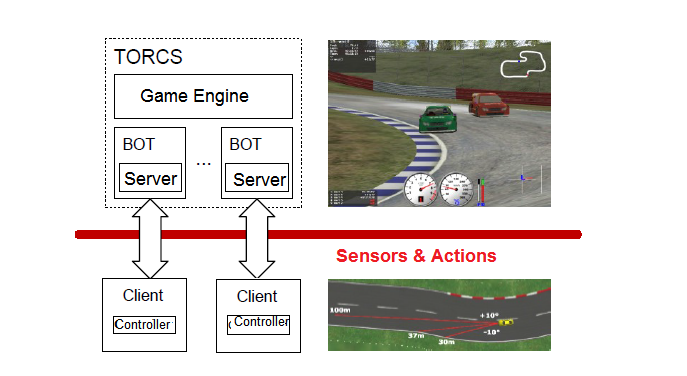
\includegraphics[width=1.1\textwidth]{fig/arch2.png}
	\begin{minipage}{10cm}
		\centering
		
		\caption{\footnotesize TORCS Architecture}
		\label{architorcs}
	\end{minipage} 
\end{figure}

\subsection{Sensors and Actuators}
The TORCS software creates a physical separation between the game engine and driver bots. So to develop a bot, it is not necessary to have any knowledge about the TORCS engine  or internal data structure.[\cite{torcs2012}]\\

In the competition, The robot perceives the racing environment through a number of sensors that provide information about the state of the car (the current speed, fuel level, ...), the state of the race (current lap, the elapsed distance,...), opponents positions and track borders, ... these data enable the designer to form a base of solutions to achieve a typical driving. [\cite{manuel}] [\cite{torcs2}]		\\		
Tables ~\ref{t1} present a complete list of available sensors with a description of each one.[\cite{Torcs3}]\\

\begin{table}[h!]
	
	\begin{tabular}{|p{2cm}|p{3cm}|p{3 cm}|p{4 cm}|}
		\hline
		{\textbf{Sensor} }&
		{\textbf{Name} }&
		{\textbf{Range} (unit)} &  
		{\textbf{Data type}}\\ 
		\hline
		1 & Angle & [-$\pi$,+$\pi$ ] & Double\\ 
		\hline
		2 & curLapTime & [0,+$\infty$) (s)	& Double\\ 
		\hline 
		3 & damage & [0,+$\infty$)(point)& Double\\ 
		\hline 
		4 & distFromStart & [0,+$\infty$) (m)& Double \\ 
		\hline 
		5 & distRaced &[0,+$\infty$) (m)& Double\\
		\hline 
		
		6 & focus & [0,200] (m)& Double\\
		\hline 
		
		7 & fuel & [0,+$\infty$) (l)& Double\\
		
		\hline
		8 & gear & \{-1,0,1,.. 6\}g& Integer \\
		
		\hline
		9 & lastLapTime &[0,+1] (s) & Double \\
		
		\hline
		10 & opponents &[0,200] (m)& Double \\
		
		\hline
		10 & racePos & \{1,2,...,N\} & Double \\
		\hline
		11 & rpm    & [0,+$\infty$) (rpm)   & Double \\
		\hline  
		13 & speedX & (-$\infty$,+$\infty$) (km/h) & Double\\
		\hline  
		14 & speedY &(-$\infty$,+$\infty$) (km/h)  & Double\\
		\hline 
		15 & speedZ & (-$\infty$,+$\infty$) (km/h) & Double \\
		
		\hline
		16 & track &  [0,200 ] & Double\\ 
		\hline
		17 & trackPos & (-$\infty$,+$\infty$) & Double\\
		
		\hline
		
		18 & wheelSpinVel  & [0,+$\infty$) (rad/s) & Double\\
		
		\hline
		19 & z &  (-$\infty$,+$\infty$) (m) & Double\\
		
		\hline
		
	\end{tabular}
	\caption{Available TORCS sensors Description}
	\label{t1}
\end{table}
\subsubsection{Actuators}
The driver bot is controlled in the game TORCS through a  typical set of actuators: the steering wheel "Steer", the accelerator "accel" the brake pedal and the gearbox. In addition, a meta-action is available to request a restart of the race to the server. Table~\ref{tab2}  details the available actions and their representation. [\cite {torcs} ]


\begin{table}[h!]
	
	\begin{tabular}{|p{3cm}|p{3 cm}|p{6 cm}|}
		\hline
		
		{\textbf{Action} }&
		{\textbf{Range} (unit)} &  
		{\textbf{Data type}}\\ 
		\hline
		Acceleration & [0,+1] & Double\\ 
		\hline
		Brake & [0,+1]	& Double\\
		\hline
		Gear & -1..0..+6	& Double\\
		\hline
		Steer & [-1,+1]	& Double\\
		\hline
		Clunch & [-1,+1]	& Double\\
		\hline
	\end{tabular}
	
	\caption{TORCS Actuators}
	\label{tab2}
\end{table}





\subsection{TORCS Controller Architecture}

A robot is a program run from TORCS that drives a car. It gets as input information about the current state of the car and its situation on the track. These collected data are used to compute actions to do in the next simulation tick; like steer, gear changes, acceleration or brake and clunch. A client may request a restart of the race by sending a special action on the server: Resatart or shutdown.
[\cite{manual}]
The basic architecture of a controller consists of 5 simple modules (fig.\ref{archi}). This modular architecture  is a key factor to achieve good results. The basics modules functions  are explained below [\cite{fuzzy}]:

\begin{figure}[h!]
	
	\centering
	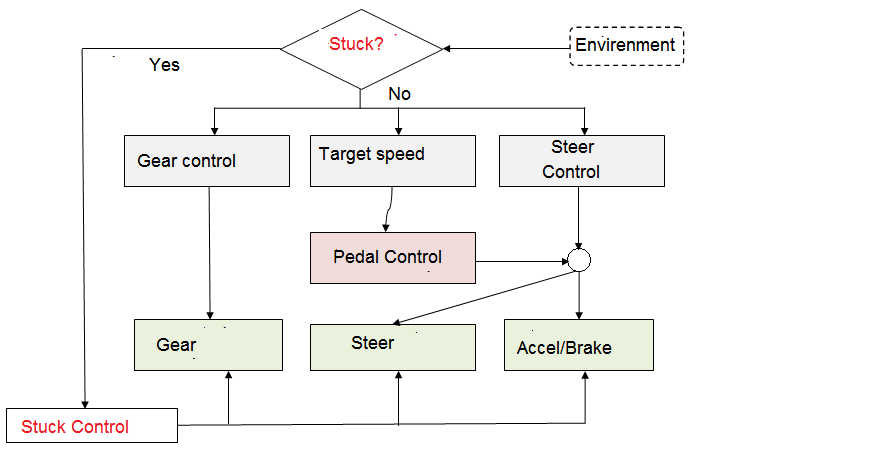
\includegraphics[width=0.9\textwidth]{fig/archicontrole2.PNG}
	\begin{minipage}{10cm}
		\centering
		\caption{\footnotesize Controller's Architecture.}
		\label{archi}
	\end{minipage} 	
\end{figure}
\newpage


\begin{enumerate}
	
	
	\item The gear control is mainly responsible for switching between first and sixth gear. Its functionality is completed with the task of detecting stuck  situations to apply the reverse.
	
	\item The target speed unit affects the speed limit for a track segment.
	
	\item speed control uses the results of others modules  to update or maintain certain speed by managing the throttle and the brake pedal. In addition, two techniques are implemented to prevent the car from slipping. A traction control (TCL) and an anti-lock anti-brake system (ABS) that will reduce, if necessary, actions over the accelerator and brake, respectively.
	
	\item Steer control module  manages the car's direction by acting on the vehicle wheel.[\cite{fuzzy}]
	\item The learning module detects segments of the track where the target speed can be increased or decreased with information on the previous laps, straight segments or segments where the car is off the track [\cite{fuzzy2}].
\end{enumerate}
\subsection{Simple driver}	
TORCS  comes with a simple driver often used to validate new designed controllers	 [\cite{torcs}][\cite{torcs2}]. \\
This project was provided by the TORCS software, and it was developed by \textit{Daniele Loiacono}  in 2007. It presents very basic functions for controlling the race car to give developers an idea of what the controller should look like. It contains simple functions to control the speed, steering angle and speed without dealing with opponents. Below are the driving principles in this system [\cite{torcs}]:\\

\begin{enumerate}
	
	
	\item 	If the car is at an angle that exceeds 30 degrees with the axis of the track  for at least 25 consecutive ticks, then it is considered in stuck.In this case, the simple driver sets the car in reverse with an angle which is the negative of the current angle. It drives the car that way at low speed until the front of the car is facing the border of the track. For example, if the car is on the left side, then it should be turned to the left. At that time, the car moves into first gear and the steering angle is reversed, so that the car can start moving forward again[\cite{torcs2}]. \\
	\item 	If the car is not in stuck, the simple driver proceeds as follows  [\cite{torcs2}]:\\
	\begin{itemize}
		\item 	First, it calculates the target speed. To do this, it gets the forward distance along the axis of the car by the front sensor FS and the sensor at 5 degrees to the left LS and 5 degrees to the right RS, as shown in Figure \ref {fig342}. Suppose RS> FS. Then, the driver made a first estimation of the "Steering angle" as the angle between the tangent to the road so that the car is facing the direction of car to the left else the angle is taken to the right. 
		
		\item Then, the target speed is calculated as follows
		
		\begin{equation}
		targetSpeed = \frac{(maxSpeed*FS*\sin(turnAngle))}{maxSpeedDist}
		\end{equation}	
		where: 	maxSpeed and maxSpeedDist are constant of the car.
		\begin{figure}[h!]
			
			\centering
			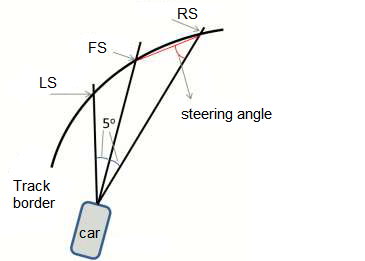
\includegraphics[width=0.7\textwidth]{fig/sensor02.png}
			\begin{minipage}{10cm}
				\centering
				\caption{\footnotesize Computing steering angle in simple driver.}
				\label{fig342}
			\end{minipage} 
		\end{figure}
	\end{itemize}		
	
\end{enumerate}


%%%%%%%%%%%%%%%%%%%%%%%%%%%  FUZZY CONTROLLER  %%%%%%%%%%%%%%%%%%%%%%%%%%%%
%
\section{Proposed Fuzzy Controller}
\label{subsec:fuzzy_controller}


The proposed controller "AD" has the same modular architecture as the simple driver where the target speed  and speed values are  computed via fuzzy controller using five 5 position sensors.
\begin{figure}[h!]
	
	\centering
	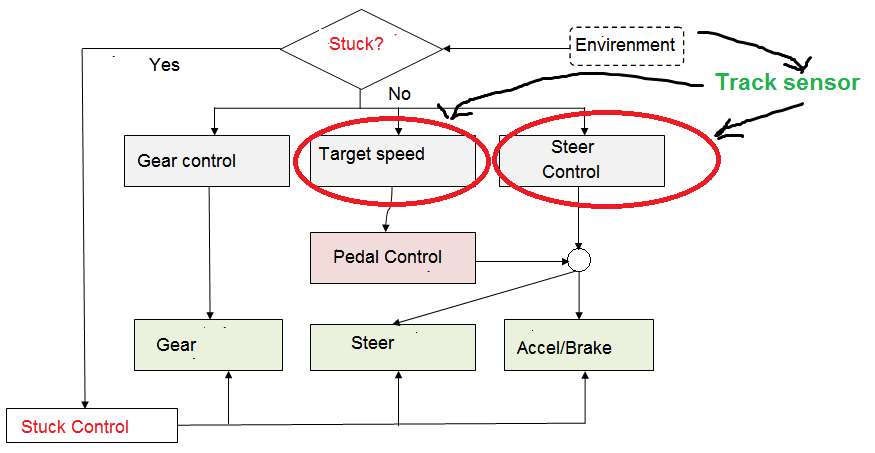
\includegraphics[width=0.8\textwidth]{fig/speedcible3.png}
	\begin{minipage}{10cm}
		\centering
		\caption{\footnotesize Target speed fuzzy control Architecture.}
		\label{archi2}
	\end{minipage} 
\end{figure}
\subsection{Fuzzy target speed}
To estimate the target speed  based on fuzzy rules, two cases are considered.
\begin{enumerate}
	\item If the car is in straight line, the target speed will take a maximum value (maxSpeed).\\\\
	\item If it is near a curve, the controller will decrease its current speed to a value included in the interval [minSpeed; maxSpeed] km / h for example if the turn is a strict turn the target speed will have a minimum value and a wide turn, it will have an average value.
	
\end{enumerate}
In case the car is off the track or near a curve, the brake system is activated, ie the ABS and TCS will be loaded to avoid the car skidding.
\\
The obtained target speed will be used in calculating the value of acceleration
(see fig.\ref{fig32} et fig.\ref{fig33}).
\\\\
\begin{equation}	
Gas(speed-Target_{speed})=-1+\frac{2}{1+e^{speed-Target_{speed}}}	
\end{equation}

Gas is for acceleration, Speed is the  current speed of the car.\\
Our fuzzy controller has 3 input values and one output: the target speed value(See figure \ref{AD}):

\begin{figure}
	\begin{center}
		
		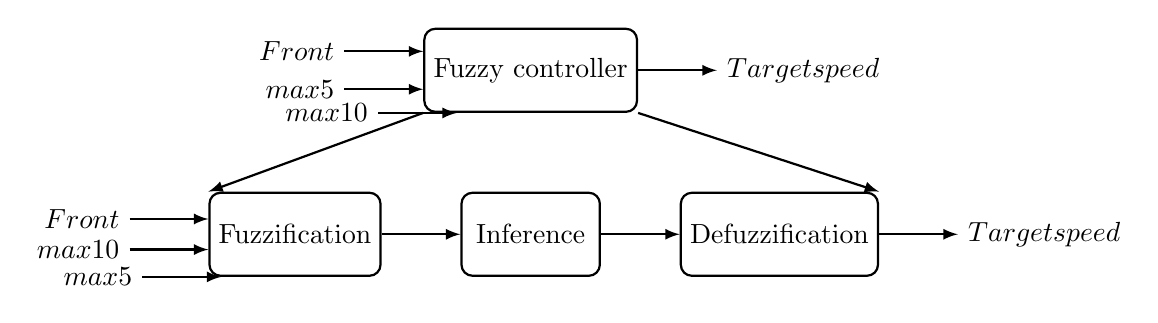
\begin{tikzpicture}[box/.style={draw, fill=white!20,rounded corners,align=center,minimum height=3em, minimum width=5em},thick,->,>= latex]
		
		\node[box] (a0) {Fuzzy controller};
		\node[left=of a0.170,font=\bfseries] (aux01) {$Front$};
		\node[left=of a0.190,font=\bfseries] (aux02) {$max 5$};
		\node[left=of a0.210,font=\bfseries] (aux03) {$max10 $};
		\node[right=of a0,font=\bfseries] (c0) {$Target speed$};
		\draw[thick,->,>= latex] (aux01) -- (a0.170);
		\draw[thick,->,>= latex] (aux02) -- (a0.190);
		\draw[thick,->,>= latex] (aux03) -- (a0.210);
		\draw[thick,->,>= latex] (a0) -- (c0);
		\node[box,below=of a0] (b) {Inference};
		
		\node[box, left=of b] (a) {Fuzzification};
		\node[left=of a.170,font=\bfseries] (aux1) {$Front$};
		\node[left=of a.190,font=\bfseries] (aux2) {$max10$};
		\node[left=of a.210,font=\bfseries] (aux3) {$max 5$};
		
		\node[box,right=of b] (b1) {Defuzzification};
		\node[right=of b1,font=\bfseries] (c) {$Target speed$};
		\draw[thick,->,>= latex] (aux1) -- (a.170);
		\draw[thick,->,>= latex] (aux2) -- (a.190);
		\draw[thick,->,>= latex] (aux3) -- (a.210);
		\draw[thick,->,>= latex] (a) -- (b);
		\draw[thick,->,>= latex] (b) -- (b1);
		\draw[thick,->,>= latex] (b1) -- (c);
		
		
		\draw[thick,->,>= latex] (a0.south west) -- (a.north west);
		\draw[thick,->,>= latex] (a0.south east) -- (b1.north east);
		
		
		\end{tikzpicture}
		
		%\includegraphics [width=10cm,height=4cm]{figures/c2/sif}
	\end{center}
	\caption{Fuzzy control of target speed.}     % width is 8.4 cm.
	\label{AD}
\end{figure}



The "AD" controller is a Mamdani based fuzzy system (See fig.\ref{AD}) with trapezoidal membership functions for input variables. It uses three values among the 19 of the track sensor (See fig.\ref{fig34}):\\

\begin{enumerate}
	\item Front = Track[9]  with angle = 0 , the front distance between the car and the border of track.
	\item M5 = max (Track[8]; Track[10])
	the max distance with +5 and  -5 angle.
	\item M10 = max (track[11]; track[7]) ,	the max distance with +10 and  -10 angle.
\end{enumerate}
\begin{figure}[h!]
	
	\centering
	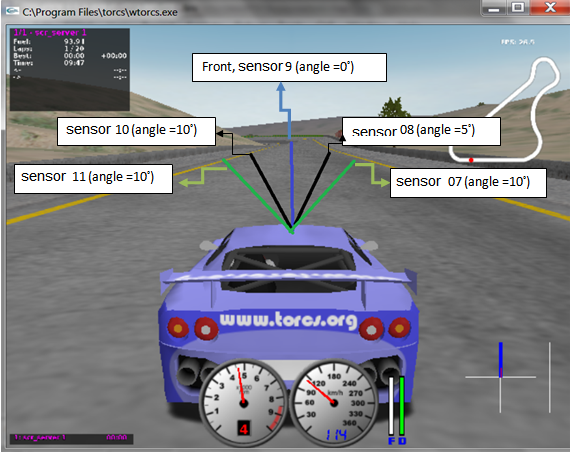
\includegraphics[width=0.9\textwidth]{fig/sensor22.png}
	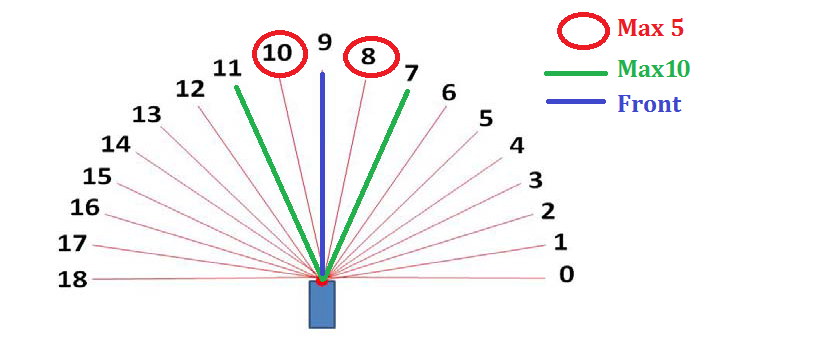
\includegraphics[width=0.9\textwidth]{fig/front.png}
	\begin{minipage}{10cm}
		\centering
		\caption{\footnotesize Fuzzy inputs.}
		\label{fig34}
	\end{minipage} 		
\end{figure}
\newpage
\begin{enumerate}
	
	\item{\textbf{Fuzzification}}
	
	Each input variable is represented by three membership functions Low, Medium
	and High as shown in the figures (fig. \ref {forehead} , Fig. \ref{max5} , fig, \ref{max15} , Fig. \ref{fontfig})\\
	The description of fuzzy inputs and output are represented in table \ref{flouevar} .\\	
	
	\begin{table} [h!] 
		\label{flouevar}
		\caption{ Fuzzy variables description}
		\begin{tabular}{ |p{1cm}|p{2cm}|p{1.5cm}|p{2 cm}|p{1 cm}|p{1.5 cm}|p{1.5 cm}|}
			\hline
			{ \color{red} Variable }&
			{ \color{red}Range }&
			{ \color{red}Name}&  
			{ \color{red} MF } &
			{ \color{red} Low } &
			{ \color{red} Medium }&
			{ \color{red} High } 
			
			\\
			\hline
			Input & [0-100] m & Front & trapezoidal & [0-50] & [20-80] &[80-100]
			\\
			\hline
			Input & [0-100] m & M5 & trapezoidal &[0-40] & [10-70] & [40-100] 
			\\
			\hline
			Input & [0-100] m  & M10 & trapezoidal & [0-30] & [0-60] & [30-100]
			\\
			\hline 
			Output & [0-200]m/s & TS & singleton & / & / & /
			\\
			\hline 
		\end{tabular} 
	\end{table}
	\begin{figure}
		\begin{center}
			
			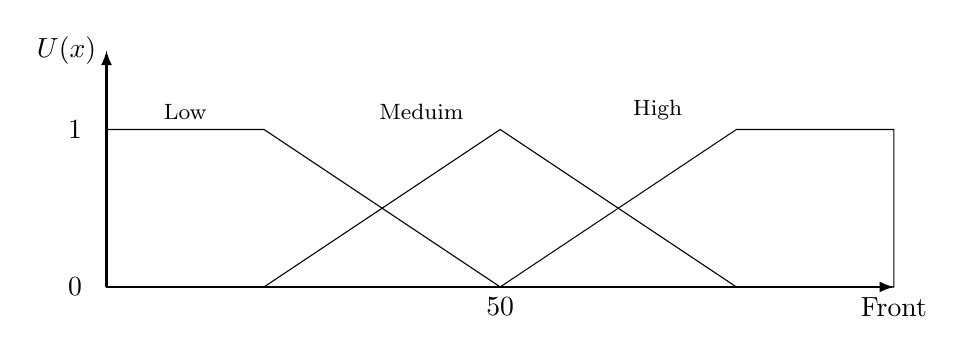
\begin{tikzpicture}[scale=2]
			%\draw[->] (0,0) -- node[below] {quantized} (4.5,0) node[below] {Age};
			%\draw[->] (0,0) -- (0,1.5) node[left] {$\mu$};
			%\node at (-0.2,0) {0};
			%\node at (-0.2,1) {1};
			%\draw[fill=yellow] (0,1) -- (4,1) -- (4,0) -- (0,0) -- cycle;
			%\foreach \x in {0.5,1,1.5,2,2.2,3.4}
			%  \draw (\x,0) -- (\x,1);
			\begin{scope}[xshift=2cm]
			\draw[thick,->,>= latex] (0,0) -- node[below] {50} (5,0) node[below] {Front};
			\draw[thick,->,>= latex] (0,0) -- (0,1.5) node[left] {$U(x)$};
			\node at (-0.2,0) {0};
			\node at (-0.2,1) {1};
			\draw (0,1) -- (1,1) -- (2.5,0) -- (0,0) -- cycle;
			\draw (1,0) -- (2.5,1) -- (2.5,1) -- (4,0) -- cycle;
			\draw (2.5,0) -- (4,1) -- (4,1) -- (5,1) -- (5,0) -- cycle;
			
			%\draw[fill=blue!40] (2.25,0) -- (3,1) -- (4,1) -- (4,0) -- cycle;
			%\draw[fill=blue!40] (1.25,0) -- (1.8,1) -- (2.3,1) -- (3,0) -- cycle;
			%\draw (1,1) -- (1.75,0) -- (2.25,0) -- (3,1);
			\node[above,font=\footnotesize] at (0.5,1) {Low};
			\node[above,font=\footnotesize] at (2,1) {Meduim};
			\node[above,font=\footnotesize] at (3.5,1) {High};
			\end{scope}
			%\node[anchor=south] at (current bounding box.north)
			%  {\textbullet\ continuous $\rightarrow$ quantized $\rightarrow$ granulated};
			\end{tikzpicture}
			%\includegraphics [width=10cm,height=4cm]{figures/c2/exemple_floue}
		\end{center}
		\caption{Membership functions of  "Front".}     % width is 8.4 cm.
		\label{front}
	\end{figure}
	\begin{figure}
		\begin{center}
			
			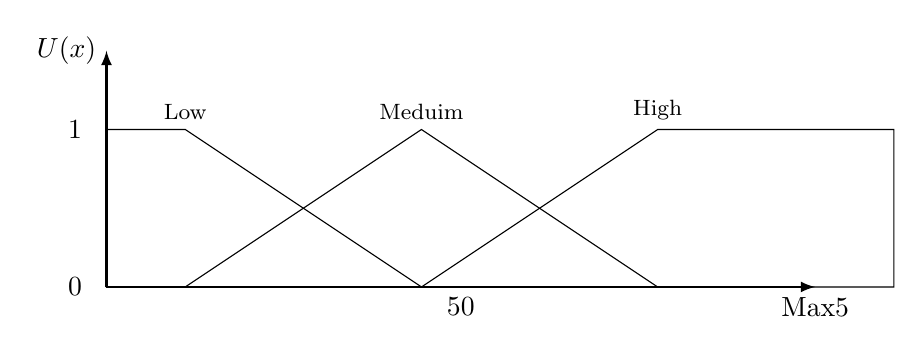
\begin{tikzpicture}[scale=2]
			%\draw[->] (0,0) -- node[below] {quantized} (4.5,0) node[below] {Age};
			%\draw[->] (0,0) -- (0,1.5) node[left] {$\mu$};
			%\node at (-0.2,0) {0};
			%\node at (-0.2,1) {1};
			%\draw[fill=yellow] (0,1) -- (4,1) -- (4,0) -- (0,0) -- cycle;
			%\foreach \x in {0.5,1,1.5,2,2.2,3.4}
			%  \draw (\x,0) -- (\x,1);
			\begin{scope}[xshift=2cm]
			\draw[thick,->,>= latex] (0,0) -- node[below] {50} (4.5,0) node[below] {Max5};
			\draw[thick,->,>= latex] (0,0) -- (0,1.5) node[left] {$U(x)$};
			\node at (-0.2,0) {0};
			\node at (-0.2,1) {1};
			\draw (0,1) -- (0.5,1) -- (2,0) -- (0,0) -- cycle;
			\draw (0.5,0) -- (2,1) -- (2,1) -- (3.5,0) -- cycle;
			\draw (2,0) -- (3.5,1) -- (3.5,1) -- (5,1) -- (5,0) -- cycle;
			\node[above,font=\footnotesize] at (0.5,1) {Low};
			\node[above,font=\footnotesize] at (2,1) {Meduim};
			\node[above,font=\footnotesize] at (3.5,1) {High};
			\end{scope}
			%\node[anchor=south] at (current bounding box.north)
			%  {\textbullet\ continuous $\rightarrow$ quantized $\rightarrow$ granulated};
			\end{tikzpicture}
			%\includegraphics [width=10cm,height=4cm]{figures/c2/exemple_floue}
		\end{center}
		\caption{Membership functions of  "Max5".}     % width is 8.4 cm.
		\label{max5}
	\end{figure}
	\begin{figure}
		\begin{center}
			
			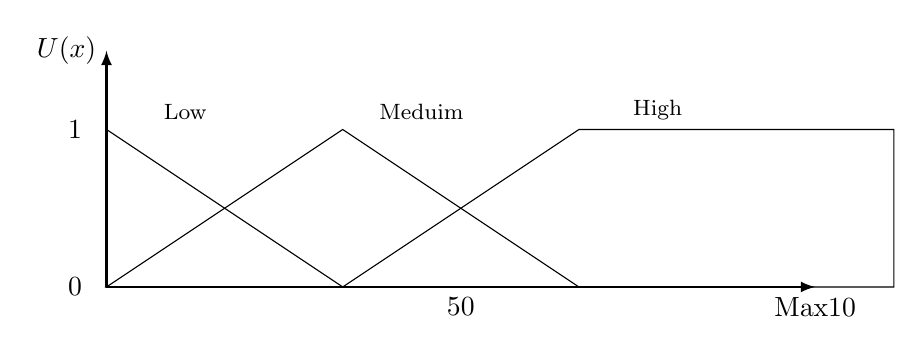
\begin{tikzpicture}[scale=2]
			%\draw[->] (0,0) -- node[below] {quantized} (4.5,0) node[below] {Age};
			%\draw[->] (0,0) -- (0,1.5) node[left] {$\mu$};
			%\node at (-0.2,0) {0};
			%\node at (-0.2,1) {1};
			%\draw[fill=yellow] (0,1) -- (4,1) -- (4,0) -- (0,0) -- cycle;
			%\foreach \x in {0.5,1,1.5,2,2.2,3.4}
			%  \draw (\x,0) -- (\x,1);
			\begin{scope}[xshift=2cm]
			\draw[thick,->,>= latex] (0,0) -- node[below] {50} (4.5,0) node[below] {Max10};
			\draw[thick,->,>= latex] (0,0) -- (0,1.5) node[left] {$U(x)$};
			\node at (-0.2,0) {0};
			\node at (-0.2,1) {1};
			\draw (0,1) -- (0,1) -- (1.5,0) -- (0,0) -- cycle;
			\draw (0,0) -- (1.5,1) -- (1.5,1) -- (3,0) -- cycle;
			\draw (1.5,0) -- (3,1) -- (3,1) -- (5,1) -- (5,0) -- cycle;
			\node[above,font=\footnotesize] at (0.5,1) {Low};
			\node[above,font=\footnotesize] at (2,1) {Meduim};
			\node[above,font=\footnotesize] at (3.5,1) {High};
			\end{scope}
			%\node[anchor=south] at (current bounding box.north)
			%  {\textbullet\ continuous $\rightarrow$ quantized $\rightarrow$ granulated};
			\end{tikzpicture}
			%\includegraphics [width=10cm,height=4cm]{figures/c2/exemple_floue}
		\end{center}
		\caption{Membership functions of  "Max10".}     % width is 8.4 cm.
		\label{max15}
	\end{figure}
	
	\begin{figure}[h!]
		
		\centering
		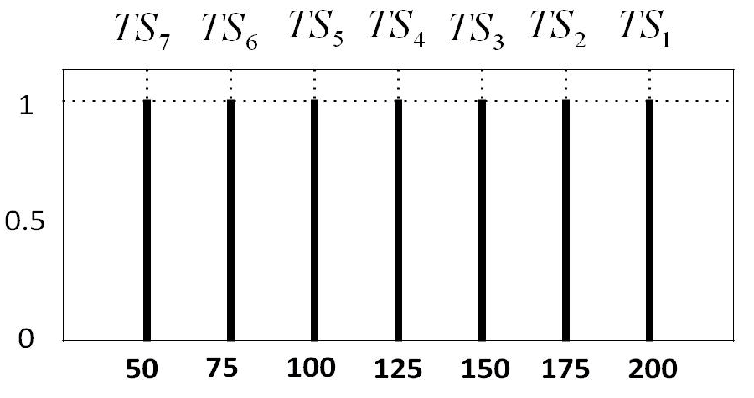
\includegraphics[width=0.7\textwidth]{fig/speed.png}
		\begin{minipage}{10cm}
			\centering
			\caption{\footnotesize Target speed values.}
			\label{fontfig}
		\end{minipage} 
		
	\end{figure}
	
	\item{\textbf{Fuzzy inference system}}
	The rules base is designed on the principle that if the front distance is maximal, then target speed should be maximal, and this value should be less when  the frontal distance is lower. The fuzzy rules are listed below:
	\\
	\begin{enumerate}
		
		
		\item If Front is High Then TargetSpeed is TS1
		\item If Front is Medium Then TargetSpeed is TS2
		\item If Front is Low and M5 is High Then TargetSpeed is TS3
		\item If Front is Low and M5 is Medium Then TargetSpeed is TS4
		\item If Front is Low and M5 is Low and M10 is High Then TargetSpeed is TS5
		\item If Front is Low and M5 is Low and M10 is Medium Then TargetSpeed is TS6
		\item  If Front is Low and M5 is Low and M10 is Low Then TargetSpeed is TS7
		\\
		In addition, a crisp rule is added to rule base to obtain a maximum value of a target speed when the value of the three input variables as far as possible, less than 100 m: \\\\
		\item If Front = Maxdistspeed or M5 = Maxdistspeed or M10 = Maxdistspeed Then TargetSpeed = Maxspeed	
		
	\end{enumerate}
	
	\item{\textbf{Deffuzzification}}
	The output value (target speed) is encoded by seven singletons.
	This phase is to transform the fuzzy set of output in a real value for the controlled system . \\
	
	\subsection{Fuzzy Steer}
	
	We can use another fuzzy controller in the control of the Steer to estimate and determine the target position of the car:\\
	if the car is straight line then it will take as target position half width of the race track.\\
	
	
	\begin{figure}[h!]
		
		\centering
		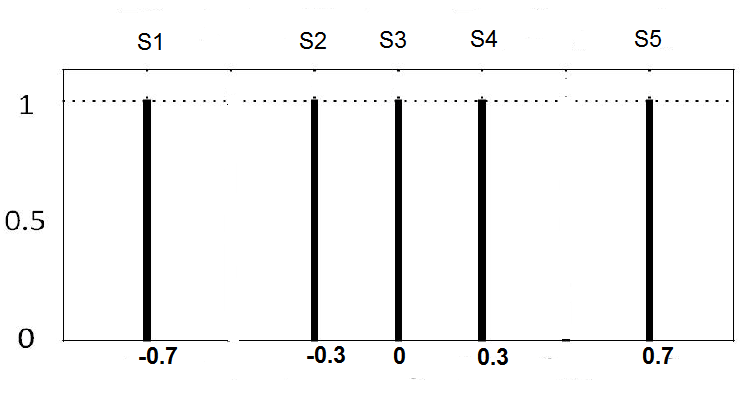
\includegraphics[width=0.4\textwidth]{fig/speed2.png}
		\begin{minipage}{10cm}
			\centering
			\caption{\footnotesize Steer values.}
			\label{fontfig6}
		\end{minipage} 
	\end{figure}
	
	
	
	If the car is near a right curve,it will approach the path leading to the right, with a space between the car and the border of the track to avoid the loss of control and shocks .The same if the car is near a left curve (see fig. \ref {steercont} ) \\
	
	Detection of curves is based on the sensor values (M10, M5, front).
	
	\begin{figure}[h!]
		
		\centering
		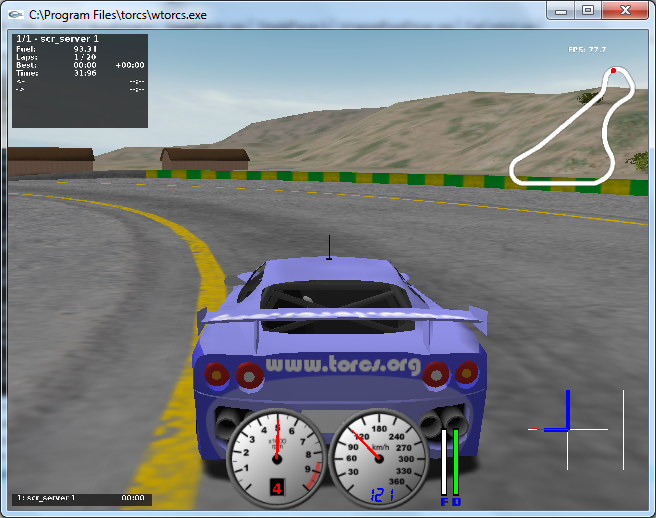
\includegraphics[width=0.5\textwidth]{fig/steercont.png}
		\begin{minipage}{10cm}
			\centering
			\caption{\footnotesize 'Steer control' of a car in a curve.}
			\label{steercont}
		\end{minipage} 
	\end{figure}
	the rule base is presented as follows:\\
	\begin{itemize}
		
		\item If Front is High Then steer is S3
		\item If Front is Medium Then steer is TS2
		\item If Front is Low and M5 is High Then steer is TS3
		\item If Front is Low and M5 is Medium Then steer is TS4
		\item If Front is Low and M5 is Low and M10 is High Then steer is TS5
		\item If Front is Low and M5 is Low and M10 is Medium Then steer is TS6
		\item  If Front is Low and M5 is Low and M10 is Low Then steer is TS7
		\\
	\end{itemize}	
\end{enumerate}

%%%%%%%%%%%%%%%%%%%%%%%%%%%%%%  RESULTS  %%%%%%%%%%%%%%%%%%%%%%%%%%%%%
%
\section{Simulation Results}
\label{subsec:results}

In this section we present all the experiments that we performed in order to measure the performance of our controller "AD".
We first, describe the methodology we have used and next, we present the experimental results of the implementation of the "AD", with opponents and
using special criteria in each case. \\


We have established a set of tests to measure the performance of the controller "AD". We compared the newly developed Controller with existing methods: the simple driver. We will run every single control car by choosing the car called "SRC-server1" in several race tracks. \\

\subsection{Simulation settings}
TORCS provides different tracks to choose from. These race tracks are designed by different developers in order to test the performance of the controllers on different difficulty circuits and on different types of roads.\\

In our case, we chose three of road tracks, a dirt road, and an oval track.\\


On oval tracks, E-Track5 (Figure \ref{fig30}) seems to be the most interesting, as it has curves in both directions. On dirt roads, Dirt1 has a good variety of curves. For road tracks, we selected three tracks: Forza, E-Road and CG-Speedway Number1. Table \ref{Tabtrack}  presents the properties and description of each selected track.\\

\begin{table}[h!]
	
	\caption{Description of Selected tracks}
	\label{Tabtrack}
	\begin{tabular}{ |p{2cm}|p{2 cm}|p{2 cm}|p{2 cm}|p{2 cm}|p{2 cm}|}
		\hline
		\textbf{Track name}    & E-Track5
		& Dir1 4 
		& Forza
		& E-Road
		& CG-Speedway Number1
		\\
		\hline
		\textbf{Shape}   
		& fig.\ref{fig3} (4)
		& fig.\ref{fig3} (2)
		& fig.\ref{fig3} (3) 
		& fig.\ref{fig3} (2)
		& fig.\ref{fig3} (1)
		
		\\
		\hline
		\textbf{Track Type}   
		& Oval
		& Dirty
		& Road
		& Road
		& Road
		
		\\
		\hline
		\textbf{Description}   
		& simple track race
		
		& Track for outdoor race
		& Very fast and smooth
		& Track race
		& rhythmic track and fast enough
		
		\\
		\hline
		
		\textbf{Length}   
		& 1621.73 m
		& 3260.43 m
		& 5784.10 m
		& 3260.43 m
		& 2057.56 m
		
		\\
		\hline
		\textbf{Width}   
		& 20.0 m
		& 16.0 m
		& 11.0 m
		& 16.0 m
		& 15.0 m
		\\
		\hline
	\end{tabular} 
\end{table}
\begin{figure}[h!]
	
	\centering
	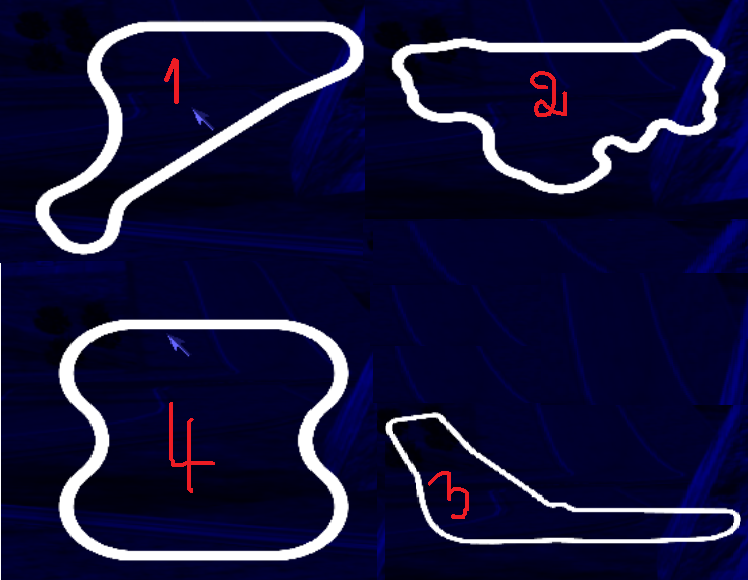
\includegraphics[width=0.7\textwidth]{fig/trackresultat.png}
	\begin{minipage}{10cm}
		\centering
		\caption{\footnotesize Tracks shape.}
		\label{fig3}
	\end{minipage} 
	
\end{figure}
\subsubsection{ Cars settings}

SCR 1 server is a NASCAR car and member of the SCR Server team (A team can used different types of car as  car1-stock1, car1-tbr1 ...).\\
A Sprint Cup Series NASCAR-type car weighs at least 1542 kg for 850 horses with . The engine is a V8 with  $ 5,866 cm ^ 3 $. Its chassis is tubular type. It has a Borg-Warner gearbox with four-speed for road circuits.\\

In our simulations, we used the car "car1-tbr1" see Fig.\ref{car} 
\begin{figure}[h!]
	
	\centering
	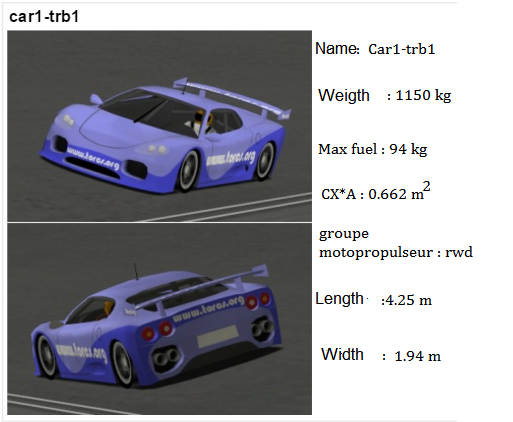
\includegraphics[width=0.8\textwidth]{fig/car1.png}
	\begin{minipage}{10cm}
		\centering
		\caption{\footnotesize car1-trb1 features  .}
		\label{car}
	\end{minipage} 
	
\end{figure}

\subsubsection{Controllers settings}
To validate the fuzzy controllers, we have considered the following controllers:\\
AD1: Fuzzy target speed  controller \\
AD2: Fuzzy steer and speed controller \\
AD5: Fuzzy target speed  controller with opponent consideration \\
SD: Simple driver \\

We conducted a series of experiments to measure the performance of the best version control in some race tracks (05 tracks in table \ref{Tabtrack} ).

\subsection{Results of 20 lap practice race}
In this case, we tested our controllers in a 20 laps practice race in the four tracks:\\
	
In this section, we set the distance to 20 laps for each track and for each controller. \\	

\begin{table} [h!] 
	
	\caption{Results for 20 laps}
	\label{resultat1}

	\begin{tabular}{ |p{3cm}|p{2cm}|p{2cm}|p{2 cm}|p{2 cm}|}
		
	\multicolumn{5}{c}{\textbf{E-Track5}}\\
		\hline
		{ \color{blue}\textbf{20 laps} }&
		{ \color{red}\textbf{SD}}&  
		{ \color{red} \textbf{AD1} } &
		{ \color{red} \textbf{AD2} } &
		{ \color{red} \textbf{AD5} }
		\\
		\hline
		Best Time & 01:05:15  & 01:21:24  &04:33:24 & 29:87 
		\\
		\hline
		Topspeed & 149  & 148 & 203 & 199 
		\\
		\hline
		Minspeed & 46 & 44 & 60 & 172 
		\\
		\hline 
		
		
		Lastlap	Time  & 01:05:17 & 01:31:36 & 01:02:55 & 30:07
		\\
		\hline 
		Best lap & 14 & 02 & 18 & 8 
		\\
		\hline
		Damage & 0 & 0 & 0 & 0 
		\\
		\hline 
		Fuel & 71:22 & 71:25 & 77:45 & 77:02 
		\\
		\hline 
		Lap & 20/20 & 20/20 & 20/20 &20/20
		\\
		\hline
\multicolumn{5}{c}{\textbf{Dirt}}\\	
		\hline
		{ \color{blue}\textbf{20 laps} }&
		{ \color{red}\textbf{SD}}&  
		{ \color{red} \textbf{AD1} } &
		{ \color{red} \textbf{AD2} } &
		{ \color{red} \textbf{AD5} }
		\\
		\hline
		Best Time & 01:12:96 & 50:43  &02:23:12  & 35:51 \\
		\hline
		Topspeed & 132  & 126 & 136 & 139 
		\\
		\hline
		Minspeed &  21 & -52 & -43 & -54 
		\\
		\hline 
		
		
		Lastlap	Time  & 01:13:08  & 02:33:43 & 02:23:12 & 01:02:91 
		\\
		\hline 
		Best lap & 14 & 07 & 01 & 5 
		\\
		\hline
		Damage &  0 & 7438 & 905 & 9274 
		\\
		\hline 
		Fuel & 65:04 & 79:26 & 79:98 & 66:06 
		\\
		\hline
		Lap & 20/20 & 14/20 & 01/20 & 20/20
		\\
		\hline
\multicolumn{5}{c}{\textbf{Forza}}\\	
		\hline
		{ \color{blue}\textbf{20 laps} }&
		{ \color{red}\textbf{SD}}&  
		{ \color{red} \textbf{AD1} } &
		{ \color{red} \textbf{AD2} } &
		{ \color{red} \textbf{AD5} }
		\\
		\hline
		Best Time & 03:03:66  & 02:39:82 & 07:14:90  & 02:20:27 
		\\
		\hline
		Topspeed & 149 & 248 & 209 & 246 
		\\
		\hline
		Minspeed & 22  & -41 & -53 & 63 
		\\
		\hline 	
		Lastlap	Time  & 03:03:66 & 02:47:26 & 09:55:62 & 02:21:23
		\\
		\hline 
		Best lap & 20 & 04 & 01 & 04 
		\\
		\hline
		Damage & 0 & 468 & 2269 & 0 
		\\
		\hline 
		Fuel & 62:61 & 71:88 & 60:55 & 60:55
		\\
		\hline 
		Lap & 20/20 & 20/20 & 04/20 & 20/20
		\\
		\hline
	\multicolumn{5}{c}{\textbf{E-Road}}\\	
		\hline
		\hline
		{ \color{blue}\textbf{20 laps} }&
		{ \color{red}\textbf{SD}}&  
		{ \color{red} \textbf{AD1} } &
		{ \color{red} \textbf{AD2} } &
		{ \color{red} \textbf{AD5} }
		\\
		\hline
		Best Time & 02:44:93  & 02:11:39 & 04:33:59 & 01:25:66 
		\\
		\hline
		Topspeed & 149  & 202 & 203 & 207 
		\\
		\hline
		Minspeed & 24  & -58 & 32& -55 
		\\
		\hline 
		
		Lastlap	Time  & 02:45:08 & 03:00:20 & 04:51:53 & 01:27:38 
		\\
		\hline 
		Best lap & 3 & 3 & 17 & 03
		\\
		\hline
		Damage & 0 & 6056 & 7309 & 2239 
		\\
		\hline 
		Fuel & 62:11 & 78:25 & 79:25 &  55:22 
		\\
		\hline  
		Lap & 20/20 & 9/20 &20/20 & 20/20
		\\
		\hline
\multicolumn{5}{c}{\textbf{CG-Speedway Number1}}\\	
		{ \color{blue}\textbf{20 laps} }&
		{ \color{red}\textbf{SD}}&  
		{ \color{red} \textbf{AD1} } &
		{ \color{red} \textbf{AD2} } &
		{ \color{red} \textbf{AD5} }
		\\
		\hline
		Best Time & 01:25:00  & 01:12:99 & 01:12:23& 53:61 
		\\
		\hline
		Topspeed & 149  & 191& 194 & 178 
		\\
		\hline
		Minspeed & 49 & 57 & 32 & -51 
		\\
		\hline 
		
		Lastlap	Time  & 01:25:01 & 01:12:99& 01:29:65 & 01:46:47 
		\\
		\hline 
		Best lap & 12 & 20 & 02 & 02  
		\\
		\hline
		Damage & 0 & 0 & 0 &  114 
		\\
		\hline 
		Fuel & 66:66 & 62:58 & 73:38 & 60:65 
		\\
		\hline 
		Lap & 20/20 & 20/20 & 03/20 & 20/20
		\\
		\hline
	\end{tabular} 
	\label{Result1r}
\end{table}

The table (\ref{Result1r} ) above shows that among the four drivers, the minimum time has been reached by the AD5 controller in each of the five tracks, this was due to the steering unit of the target. The target position allows the car to adjust safely the required steering angle  with the maximum speed so the controller AD5 gave the best time.
\\
However, taking a smaller target angle required a greater distance to cover by car by taking a less efficient trajectory. In addition, the number of times the car was off the road on Dir1 and Forza was higher for AD5 and, accordingly, the time that the car has passed out of the track was potentially higher than the other controllers.
\\	

Thus, higher damages happened after the collision with the outer walls of the track when the car is off the track. The simple driver SD driver and AD1, AD2 especially got less damage compared the version of AD5. The simple SD driver finished the race without damage, while AD5 was able to complete all the tracks safely except the Dir1t4 and Forza circuit where the damage is a little high for the AD1 driver (fig.\ref{resultat1}) .But the result may be more favourable than the other results by SD, DA1, DA2.\\
For the fuel consumption, it  depends on  shocks rate and category of tracks.

\subsection{Time trial race}
Now, we set the race stopping criterion to 300s.
we got the results that are shown in Table  \ref{resulta9}.
\begin{table} [h!] 
	
	\caption{Results of the controllers in 5 minute time trial race}
	\label{resulta9}
	\begin{tabular}{ ||p{3cm}||p{3cm}||p{3cm}||p{3 cm}||}	
		\multicolumn{4}{c}{\textbf{E-Track5}}\\	
		
		\hline
		{ \color{blue}\textbf{} }&
		{ \color{red}\textbf{Best Time} }&
		{ \color{red} \textbf{Distance } } &
		{ \color{red} \textbf{Top speed} }
		\\
		\hline
		AD1 &01:11:98  &4540,844&  155
		\\
		\hline
		AD2 & 02:15:26 &8803,161& 155
		\\
		\hline 
		AD5 & 29:30&32600&199 
		\\
		\hline 
		\multicolumn{4}{c}{\textbf{Dir1}}\\			
		\hline
		{ \color{blue}\textbf{} }&
		{ \color{red}\textbf{Best Time} }&
		{ \color{red} \textbf{Distance } } &
		{ \color{red} \textbf{Top speed} }
		\\
		\hline
		AD1 & 52:27 & 7825,032&126  
		\\
		\hline
		AD2 & 00:00 &5202,99& 134
		\\
		\hline 
		AD5 & 00:00 &620,25& 153 
		\\
		\hline 
		\multicolumn{4}{c}{\textbf{Froza}}\\		\hline
		{ \color{blue}\textbf{} }&
		{ \color{red}\textbf{Best Time} }&
		{ \color{red} \textbf{Distance(m) } } &
		{ \color{red} \textbf{Top speed(m/s)} }
		\\
		\hline
		AD1 & 02:49:12  &17352,3  &  247
		\\
		\hline
		AD2 & 02:49:12  & 17354,12 & 239
		\\
		\hline 
		AD5 & 57:66 & 17355,2 & 203 
		\\
		\hline 
	\multicolumn{4}{c}{\textbf{E-Road}}\\	
		\hline
		{ \color{blue}\textbf{} }&
		{ \color{red}\textbf{Best Time} }&
		{ \color{red} \textbf{Distance } } &
		{ \color{red} \textbf{Top speed} }
		\\
		\hline
		AD1 & 03:62:33 & 11586,2 &  160
		\\
		\hline
		AD2 & 02:41:41  & 11588 & 208 
		\\
		\hline 
		AD5 & 01:15:16 & 23139 & 217
		\\
		\hline 
			\multicolumn{4}{c}{\textbf{CG-Speedway Number1}}\\
		\hline
		{ \color{blue}\textbf{} }&
		{ \color{red}\textbf{Best Time} }&
		{ \color{red} \textbf{Distance } } &
		{ \color{red} \textbf{Top speed} }
		\\
		\hline
		AD1 & 01:15:19 & 23136 &  195
		\\
		\hline
		AD2 & 01:15:80 & 17352,2 & 193 
		\\
		\hline 
		AD5 & 44:67& 28921,6 &206 
		\\
		\hline 
		
	\end{tabular}
\end{table}

\subsection{Real race}
\subsubsection{5 laps race}
In this case, we test our controller "AD5", without considering the variables and opponents sensors.\\

Our main goal is to test the performance of "AD5" in a race, and answer the following questions: Could we have a perfect driving in a race with "AD5" only with the track borders sensors? Can we win the race with AD5?\\
In this context we tested "AD5" in 5 tracks against berwin,bt, damned, inferno and tita teams.
\\

After the launch of the race "AD5" against the 10 cars of each team (list in table \ref{resultat30}) for 5 laps in each track we obtained the following results (see table \ref{resultat31})
\begin{table}[h!]
	\caption{Results of AD5  in a real race}
	\label{resultat31}
	\begin{tabular}{ |p{3cm}|p{2cm}|p{2cm}|p{2 cm}|p{2 cm}|p{2 cm}|}
		\hline
		{ \color{blue}\textbf{E-Track5} }&
		{ \color{red}\textbf{Against berwin team }}&  
		{ \color{red} \textbf{Against bt team} } &
		{ \color{red} \textbf{Against damned team} } &
		{ \color{red} \textbf{Against inferno team} }&
		{ \color{red} \textbf{Against tita team} }
		\\
		\hline
		Ranking & 1/11 & 2/11   & 1/11 & 7/11& 4/11
		\\
		\hline
		race time & 02:36:78 & 02:40:38+ 03:41   & 02:42:73 & 02:15:81 + lap & 02:18:74 + 28:19
		\\
		\hline
		Best time & 29:90 & 30:28   & 30:28 & 30:59& 30:53 
		\\
		\hline 
		Maxspeed & 198 & 198 &  198 & 199 & 198
		\\
		\hline
		
		Damage & 2267 & 7939 &  5888 & 5232& 8043
		\\
		\hline 
		
		
		Pit stops & 0& 0  & 0 & 0 & 0
		\\
		\hline 	
		Lap & 5/5 & 5/5  & 5/5 & 4/5 & 5/5
		\\
		\hline
		\hline
		{ \color{blue}\textbf{Froza} }&
		{ \color{red}\textbf{Against berwin team }}&  
		{ \color{red} \textbf{Against bt team} } &
		{ \color{red} \textbf{Against damned team} } &
		{ \color{red} \textbf{Against inferno team} }&
		{ \color{red} \textbf{Against tita team} }
		\\
		\hline
		Ranking & 10/11  & 11/11 & 11/11 & 10/11& 10/11
		\\
		\hline
		Race time & 7:44:99 + Lap & 8:07:39 + 02:16:32 & 08:09:42 + 1Lap & 6:40:33 + Lap 0 &  6:37:02 + Lap 
		\\
		\hline
		Best time & 01:57:58 & 01:45:30 & 02:03:00 & 02:04:00& 02:04:37
		\\
		\hline 
		Maxspeed & 243  & 282 & 260 & 220& 217
		\\
		\hline
		
		Damage & 2275 & 95 & 475 & 416 & 1185
		\\
		\hline 
		
		
		Pit stops & 0 & 0 & 0 & 0 & 0
		\\
		\hline 
		Lap & 4/5 & 5/5  & 4/5 & 4/5& 4/5 
		\\
		\hline	
	\end{tabular} 
	
\end{table}

From Table \ref {resultat31}, we noticed that our controller has won a race only in some types of tracks such as "E-track5" category "Oval track".\\

When our controller is in parallel with his opponent, and the distance between them is smaller, and they are in a smaller width track,  there is a possibility of  damage.
\\

According to damage results, despite our controller can win the race on the E-track5 but it had a higher crash rates in the majority of cases. We observed also that in the majority of cases our car is very slow compared to the other cars in each team. \\
%%%%%%%%%%%%%%%%%%%%%%%%%%%%%  CONCLUSIONS  %%%%%%%%%%%%%%%%%%%%%%%%%%%%
%
\section{Conclusions and Future Work}
\label{subsec:conclusions}




%%%%%%%%%%%%%%%%%%%%%%%%%%%%%%%%%%%%%%%%%%%%%%%%%%%%%%%%%%%%%%%%%%%%%%%

\section*{Acknowledgments}

Omitted for Blind reviews.

%This work has been supported in part by projects 
%EPHEMECH (TIN2014-56494-C4-3-P, Spanish Ministerio de Econom�a y Competitividad), 
%PROY-PP2015-06 (Plan Propio 2015 UGR), 
%PETRA (SPIP2014-01437, funded by Direcci�n General de Tr�fico),
%CEI2015-MP-V17 (awarded by CEI BioTIC Granada), and 
%PRY142/14 (funded by Fundaci�n P�blica Andaluza Centro de Estudios Andaluces en la IX Convocatoria de Proyectos de Investigaci�n).


\bibliographystyle{splncs03}
\bibliography{fuzzy_torcs}



\end{document}
